\chapter{Laboratorio 1}
In questa esperienza di laboratorio si è realizzato e analizzato il seguente circuito:
\begin{figure}[h!]
	\centering
	\begin{circuitikz}[scale=1.2, transform shape]
		\draw (0,0.5) node[ground]{};
		\draw (0,2) node[above]{$v_{in}$} to[short, o-] (0,1.5) to[sV=500<\milli\volt>] (0,0.5);
		\draw (0,2) to[R=4.7<\kilo\ohm>, -*] ++(3,0) ++(0.1,-.1) node[below]{$V^-$};
		\draw (3,2) to (4,2);
		\draw (3.7,2) node[op amp, anchor=-](oa){\texttt{TL071}};
		\draw (3.7,1) node[ground]{} to[short, -*] (3.7,1);
		\draw (3,2) -- ++(0,1.3) coordinate(C) to[C=300<\pico\farad>] ++(3.08,0) (C-|oa.out) coordinate(Co) -- (oa.out) to [short, *-o] ++(1,0) node[above]{$v_{out}$};
		\draw (3,3.3) -- ++(0,1.3) to[R=47<\kilo\ohm>] ++(3,0) -| (Co);
	\end{circuitikz}
	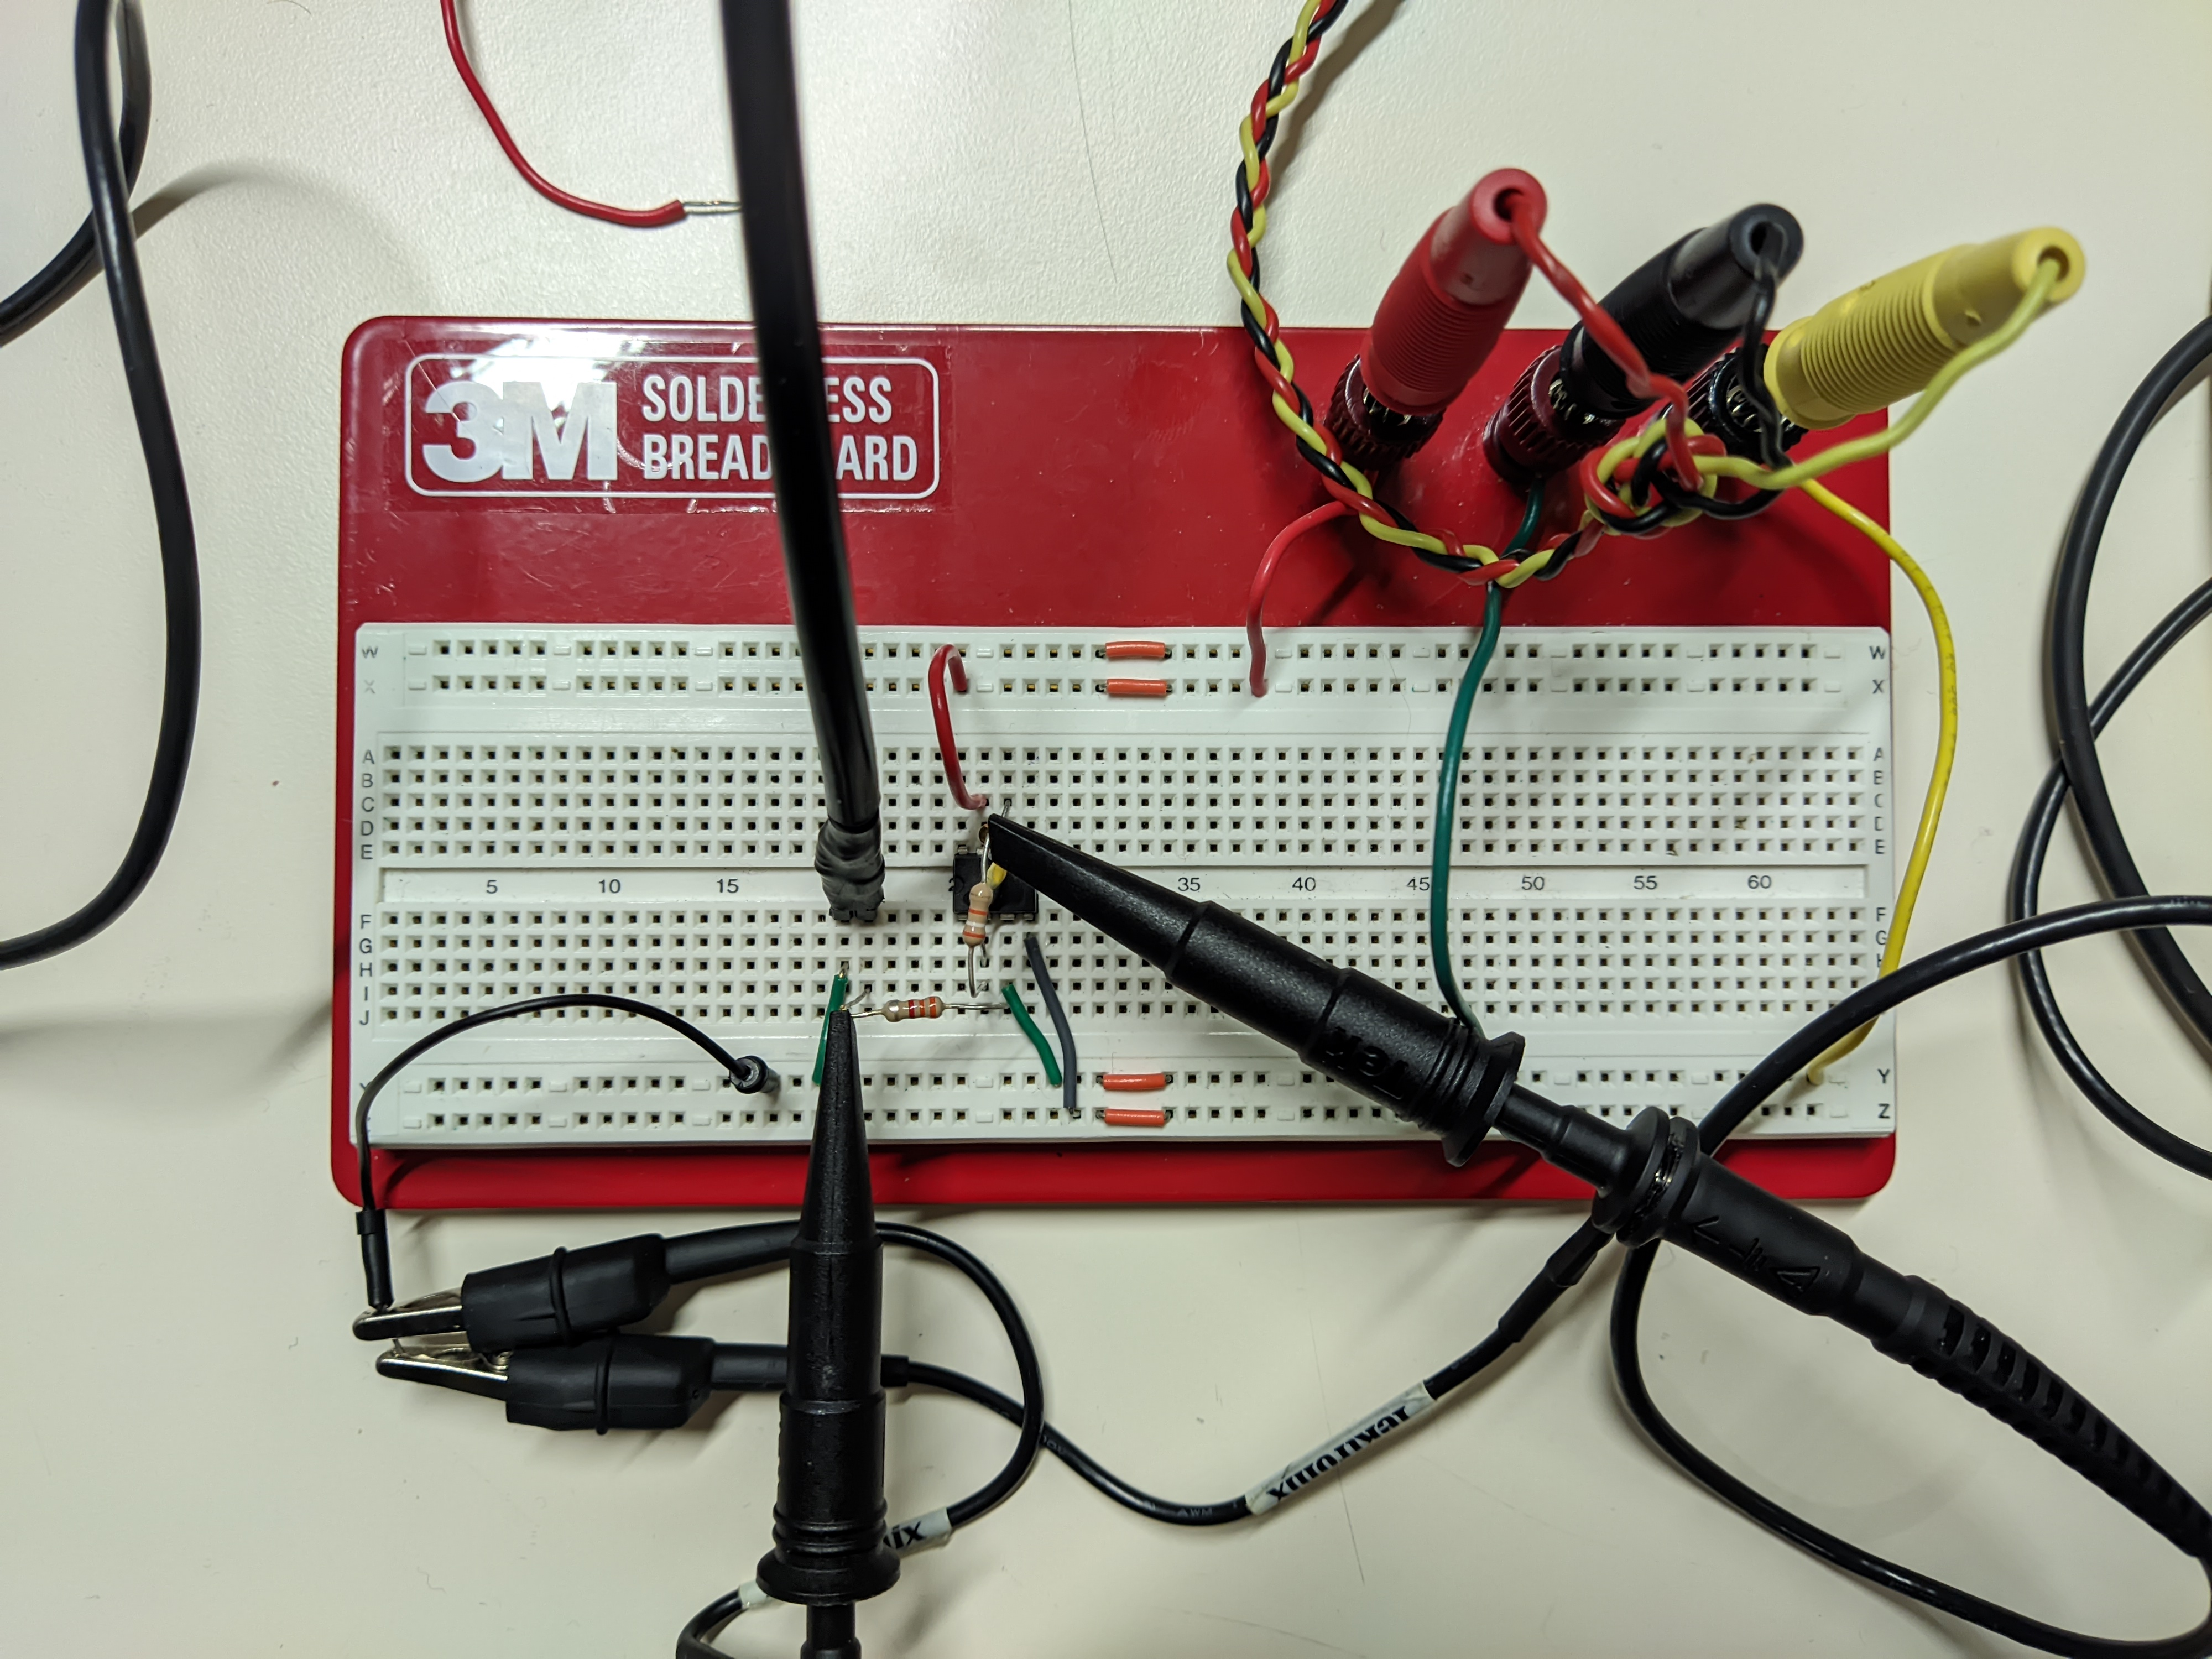
\includegraphics[width=0.4\linewidth]{./ImageFiles/Laboratorio 1/CIRC.jpg}
	\caption{Schema circuitale e foto circuito}
	\label{fig:circuito}
\end{figure}

Il circuito realizza un filtro passa basso attivo, utilizzando un amplificatore operazionale retroazionato negativamente. Infatti, è possibile ricavare la funzione di trasferimento del circuito tramite un bilancio delle correnti al nodo V\super{-}. Si consideri v\sub{in} come un generatore ideale di tensione applicato in ingresso al circuito. Indicando con Z\sub{1} l'impedenza equivalente del parallelo tra R\sub{1} e C\sub{1} e con Z\sub{2} l'impedenza della resistenza R\sub{2}, si può ottenere la funzione di trasferimento del circuito:
\begin{equation}
	v_{out}=-\frac{Z_1}{Z_2}v_{in}=-\frac{1}{R_2}\frac{R_1}{1+j w R_1 C_1} vin,
\end{equation}
da cui si ricava
\begin{equation}
	T=\frac{v_{out}}{v_{in}}=-\frac{R_1}{R_2}\frac{1}{1+j w R_1 C_1}.
\end{equation}
Questa funzione di trasferimento corrisponde a un filtro passa basso. Infatti, è possibile calcolare l'andamento del modulo e della fase in funzione di $\omega$:
\begin{equation}
	\begin{split}
		|T|&=\frac{R_1}{R_2}\frac{1}{\sqrt{1+(wR_1C_1)^2}} \\
		\angle T&=\SI{180}{\degree}-arctan(\omega R_1 C_1).
	\end{split}
\end{equation}
Per comprendere il comportamento del modulo e della fase in funzione della frequenza del segnale applicato in ingresso, è necessario analizzare i termini dipendenti da $\omega$ nelle due equazioni. Per quanto riguarda l'espressione del modulo della funzione di trasferimento, il termine $\sqrt{1+(wR_1C_1)^2}.... $ \todo{inserire le due frecce per i limiti} mentre nell'espressione della fase, il termine $arctan(\omega R_1 C_1)....$ \todo{ut supra}. Il modulo quindi tende a $\frac{R_1}{R_2}$ per segnali in ingresso a bassa frequenza, mentre tende a zero per segnali in ingresso ad alta frequenza, mentre la fase è pari a circa \SI{180}{\degree} per segnali a bassa frequenza, e tende a \SI{90}{\degree} per segnali ad alta frequenza.\todo{da sistemare questa parte}
Si determina quindi un comportamento di un filtro passa basso invertente del primo ordine, con frequenza di taglio pari a $f=\frac{1}{2\pi R_1C_1}$.

I valori dei componenti passivi sono stati scelti per soddisfare i requisiti di prestazioni del filtro. In particolare, veniva richiesto un guadagno di un fattore 10 con frequenza di taglio pari a \SI{10}{\kilo\hertz}. I valori scelti ... (\todo{inserire tabella valori con valori nominali/misurati dei componenti}).

\todo{Inserire grafici matlab}
\todo{inserire prove di saturazione}
\todo{inserire prove di offset}